\section{Introduction}

The use of spatial data structures is ubiquitous in many spatial applications, ranging from spatial databases to computational geometry, robotics, and geographic information systems \cite{samet_design_1990}. Spatial data structures have been used to improve the efficiency of various spatial queries, spatial joins, nearest neighbors, Voronoi diagrams, and robot motion planning. Examples include grids \cite{nievergelt_grid_1984}, R-trees \cite{guttman_r-trees_1984, beckmann_r-tree_1990}, and quadtrees \cite{finkel_quadtrees_1974}.  \textit{Edge-list} structures are also typically utilized in applications as topological computations in computational geometry \cite{berg_computational_2008}.

The most commonly used data structure in the edge-list family is the \textit{Doubly Connected Edge List (DCEL)}. A DCEL \cite{muller_finding_1978, preparata_computational_1985} is a data structure that collects topological information for the edges, vertices, and faces contained by a surface in the plane. The DCEL and its components represent a planar subdivision of that surface. In a DCEL, the faces (polygons) represent non-overlapping areas of the subdivision; the edges are boundaries that divide adjacent faces; and the vertices are the point endings between adjacent edges (see Figure \ref{fig:dcel_example}).  In addition to providing geometric and topological information, a DCEL can be enhanced to provide further information. For instance, a DCEL storing a thematic map for vegetation can also store the type and height of the trees around the area \cite{berg_computational_2008}.

\begin{figure}
    \centering
    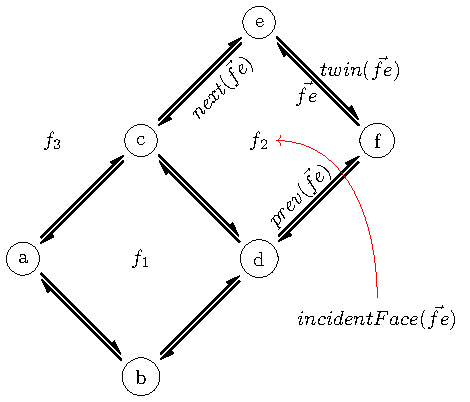
\includegraphics[width=0.6\linewidth]{chapterSDCEL/dcel_example}
    \caption{Components of the DCEL structure.}\label{fig:dcel_example}
\end{figure}

The DCEL data structure has been used in various applications. For instance, the use of connected edge lists is cardinal to support polygon triangulations and their applications in surveillance (the Art Gallery Problem \cite{chvatal_combinatorial_1975, orourke_art_1987}) and robot motion planning (\cite{berg_computational_2008, chew_convex_1993}). DCELs are also used to perform polygon unions (for example, on printed circuit boards to support the simplification of connected components in an efficient manner \cite{fogel_cgal_2012}) as well as the computation of silhouettes from polyhedra \cite{fogel_cgal_2012, berberich_arrangements_2010} (applied frequently in computer vision and 3D graphics modeling \cite{boguslawski_modelling_2011}).

Edge-list data structures have also been utilized to create thematic \textit{overlay maps}. In this problem, the input contains the DCELs of two polygonal layers, each capturing geospatial information and attribute data for different phenomena, and the output is the DCEL of an overlay structure that combines the two layers into one. In many application areas, such as ecology, economics, and climate change, it is important to be able to join the input layers and match their attributes in order to unveil patterns or anomalies in data that can be highly impacted by location. Several operations can then be easily computed given an overlay; for instance, the user may want to find the \textit{intersection} between the input layers (e.g., corresponding to soil types and evapotranspiration of plants), identify their \textit{difference} (or symmetric difference), or create their \textit{union}. 

Spatial databases use spatial indexes (R-tree \cite{guttman_r-trees_1984, beckmann_r-tree_1990}) to store and query polygons. Such methods use the \textit{filter and refine} approach where a complex polygon is abstracted by its Minimum Bounding Rectangle (MBR); this MBR is then inserted in the R-tree index. Finding the intersection between two polygon layers, each indexed by a separate R-tree, is then reduced to finding the pairs of MBRs from the two indexes that intersect (filter part). This is followed by the refine part, which, given two MBRs that intersect, needs to compute the actual intersections between all the polygons these two MBRs contain. While MBR intersection is simple, computing the intersection between a pair of complex real-life polygons is a rather expensive operation (a typical 2020 US census tract is a polygon with hundreds of edges).  Moreover, using DCELs for overlay operations offers the additional advantage that the result is also a DCEL, which can be directly used for subsequent operations. For example, one may want to create an overlay between the intersection of two layers with another layer, and so on.

Even though the DCEL has important advantages for implementing overlay operations, current approaches are sequential in nature. This is problematic, considering layers with thousands of polygons. For example, the layer representing the 2020 US census tracts contains around 72K polygons; the execution for computing the overlay over such a large file crashed on a stock laptop. To the best of our knowledge, there is no scalable solution for computing overlays over DCEL layers.

%% Extension
% In addition to the scalability issue, it is common in some applications that spatial polygons are provided in the form of scattered line segments, e.g., a set of road segments that form city blocks.  Such data can be very large and appear in applications in urban planning, geo-targeted advertising, economic and demographic studies, etc.  Yet, existing polygon overlay techniques cannot handle them directly at scale.  In that setting, extracting the DCEL subdivision's faces (polygons) is not straightforward.  To generate all of a subdivision's faces, the DCEL constructor must invoke a scalable \textit{polygonization} procedure, which extracts all closed polygons formed by a collection of planar line segments in a subdivision.

This chapter describes the design and implementation of a \textit{scalable} and \textit{distributed} approach to compute the overlay between two DCEL layers. We first present a partitioning strategy that guarantees that each partition collects the required data from each layer DCEL to work independently, thus minimizing duplication and transmission costs over 2D polygons. In addition, we present a merging procedure that collects all partition results and consolidates them in the final combined DCEL.

%% Extension
%Furthermore, we extend the overlay method to support input polygons in scattered line segments form by integrating a scalable and distributed polygon extraction approach.  Our solutions have been implemented in a parallel framework (i.e., Apache Spark).

Implementing a distributed overlay DCEL creates novel problems. First, there are potential challenges that are not present in the sequential DCEL execution. For example, the implementation should consider \textit{holes}, which could lay on different partitions, and they need to be connected with their components residing in other partitions so as not to compromise the combined DCEL's correctness.

%% Extension
%It should also consider the \textit{dangle} and \textit{cut edges} resulting from the polygonization process and their intersection with other polygon layers.

Secondly, once a distributed overlay DCEL has been built, it must support a set of binary overlay operators (namely \textit{union, intersection, difference} and \textit{symmetric difference}) in a transparent manner.  That is, such operators should take advantage of the scalability of the overlay DCEL and be able to run also in a parallel fashion. Additionally, users should be able to apply the various operators multiple times without rebuilding the overlay DCEL data structure.  

%% Extension
%This chapter extends the previous work in \cite{calderon_scalable_2023}. The main new contributions are summarized as follows. First, we introduce a new spatial partitioner, based on the kd-tree partitioning strategy, for constructing overlay  DCELs (section \ref{sec:kdtreestrategy}). Since it better utilizes the data  distributions in optimizing DCEL partitions, it leads to noticeably improved performance. The new partitioning strategy contrasts with the original strategy that employed space-partitioning techniques based on quadtrees. Second, we enable overlay DCELs to take scattered and noisy line segments as input instead of being limited to clean polygon data.  This builds on the work on scalable polygonization in \cite{abdelhafeez_ddcel_2023} to enable overlays of real datasets that consist of massive sets of line segments that cannot currently be handled by any existing technique. We also provide additional experiments, to quantify the benefits of the kd-tree based strategy, as well as the performance on the datasets with large volumes of line segments.

The rest of this chapter is organized as follows. Section \ref{sec:related} presents related work, while Section \ref{sec:prelim} discusses the basics of DCEL and the sequential algorithm. In Section \ref{sec:methods}, we present the partitioning schemes that enable parallel implementation of the overlay computation among DCEL layers; we also discuss the challenges presented in the DCEL computations by distributing the data and how to solve them efficiently. Two important optimizations are introduced in Section \ref{sec:alternative_methods}. Finally, an extensive experimental evaluation appears in Section \ref{sec:experiments}.

%% Extension
%Section~\ref{sec:polygonization} details the polygon extraction process for line input adaptation. It also extends the overlay method by supporting the overlay of dangle and cut edges.
